\chapter{Fundamentos teóricos}

\section{El mundo y la maquina}
El modelo del mundo y la máquina de Michael Jackson \cite{MundoMaquina} es una abstracción que permite formular rigurosamente algunas nociones
fundamentales de la ingeniería de requerimientos. En este modelo, los fenómenos son hechos, situaciones o eventos cuya
existencia puede observarse, la maquina es una porción del sistema a desarrollar o modificar y el mundo es una porción de
la realidad afectada por la máquina. El mundo y la máquina interactúan en la interfaz de la máquina. Un problema del mundo 
describe una parte del mundo real que nosotros queremos mejorar construyendo la solución como una máquina.

\vspace{\baselineskip} 
En este modelo, los requerimientos R son declaraciones prescriptivas (propiedades deseadas que pueden cumplirse o no) sobre 
el mundo expresadas en términos de fenómenos sobre la interfaz entre la máquina que queremos construir y el mundo en el cual 
viven los problemas que queremos resolver. Los requerimientos deben ser forzados por la maquina independientemente de cómo 
se comporte el mundo. Los problemas del mundo son capturados como declaraciones prescriptivas expresadas en término de 
fenómenos del mundo llamados objetivos G, y declaraciones descriptivas (propiedades sobre el sistema que se mantienen 
independientes a cómo se comporta el sistema) sobre lo que nosotros asumimos que es verdad en el mundo, suposiciones 
de dominio D. Las suposiciones de dominio podrían no mantenerse y deben ser satisfechas por el mundo. 

\vspace{\baselineskip}
La tarea clave de la ingeniera de requerimientos es comprender y documentar los objetivos y las características del entorno.
Teniendo estos modelos se pueden formular un conjunto de requerimientos para la máquina de forma que en conjunto con el
entorno satisfagan los objetivos. Más formalmente R, D $\vDash$ G.
Esto puede ser formulado como un problema de síntesis \cite{Sintesis}. Dados un conjunto de suposiciones del dominio y un conjunto de
objetivos del sistema, construir  automáticamente un modelo operacional de la maquina tal que compuesto con el modelo del
entorno, los objetivos sean alcanzados.

\vspace{\baselineskip}
Diremos que un evento es controlable si es controlable por la máquina. Una evento es monitoreable o no controlable si es
controlable por el mundo. 
Para cumplir los objetivos, el modelo operacional restringe la ocurrencia de eventos controlables basándose en la observación
de los eventos que ya ocurrieron.
Este problema se conoce como el problema de síntesis de controladores y está siendo estudiado exhaustivamente en varios
aspectos de la ingeniería de los requerimientos.

\section{Labelled Transition Systems}
Los Labelled Transition Systems \cite{LTS} (LTSs) son ampliamente utilizados para modelar y analizar el comportamiento de sistemas
concurrentes y distribuidos. Son un sistema de transición de estados en el cual las transiciones son etiquetadas con
acciones. El conjunto de acciones de un LTS se conoce como alfabeto comunicacional y constituye las interacciones que
el sistema modelado puede tener con el entorno.

\begin{definition}{(Labelled Transition System)}
Sea $Estados$ el conjunto universal de estados y $Acciones$ el conjunto universal de etiquetas de acciones. Un Labelled
Transition System es una tupla $E = (S_{E}, A_{E}, \Delta_{E}, s_{0}^{E})$ en donde $S_{E} \subseteq Estados$ es un conjunto
finito de estados, $A_{E} \subseteq Acciones$ es un alfabeto finito, $\Delta_{E} \subseteq (S_{E}$ x $A_{E}$ x $S_{E})$ es una
relación de transición y $s_{0}^{E} \subseteq S_{E}$ es el estado inicial.
\end{definition}

Dado $(s, l, s$’$) \subseteq \Delta_{E}$ decimos que $l$ está habilitada desde $s$ en $E$. Decimos que un LTS es
determinístico si desde un estado, al realizar una acción, hay solo un estado posible al que llegamos.

\section{Composición en paralelo}

Sean $M$ y $E$ dos LTSs. La composición en paralelo $\parallel$ es un operador simétrico que crea un nuevo LTS $M \parallel E$, 
tal que sus estados son el producto cartesiano de los estados de $M$ y $E$, sus acciones la unión de las acciones de $M$ y $E$, 
y su función de transición sincroniza el movimiento de las dos máquinas en las acciones compartidas, mientras que se 
mueven independientemente en sus acciones propias.

\begin{definition}{(Composición en paralelo)}
Sean $M = (S_{M}, A_{M}, \Delta_{M}, s_{0}^{M})$ y\\
$N = (S_{N}, A_{N}, \Delta_{N}, s_{0}^{N})$ dos LTSs. Composición en paralelo $\parallel$ es un operador simétrico tal que 
$M \parallel N$ es el LTS $P = (S_{M}$ x $S_{N}, A_{M} \cup A_{N}, \Delta_{P}, (s_{0}^{M}, s_{0}^{N}))$, donde $\Delta_{P}$ es
la menor relación que satisface las siguientes reglas:

\vspace{\baselineskip}
$\dfrac{(s, l, s') \in \Delta_{M}}{((s, t), l, (s', t)) \in \Delta_{P}}$ con $l \in A_{M} \setminus A_{N}$

\vspace{\baselineskip}
$\dfrac{(t, l, t') \in \Delta_{N}}{((s, t), l, (s, t')) \in \Delta_{P}}$ con $l \in A_{N} \setminus A_{M}$

\vspace{\baselineskip}
$\dfrac{(s, l, s') \in \Delta_{M}, t, l, t') \in \Delta_{N}}{((s, t), l, (s', t')) \in \Delta_{P}}$ con $l \in A_{M} \cap A_{N}$
\end{definition}

\section{LTS Legal}
Dados dos LTSs $N$ y $M$, y $A_{N_{u}} \subseteq A_{N}$, decimos que $M$ es un Legal LTS para $N$ respecto a $A_{N_{u}}$ si por cada
estado en $E\parallel$$M$, realizar una acción perteneciente a $A_{N_{u}}$ es igual a realizar la acción en $N$.
Intuitivamente, en la composición una acción es deshabilitada si y solo si también es deshabilitada en el LTS original.
En otras palabras, $M$ no restringe a $N$ respecto a $A_{N_{u}}$.

\begin{definition}{(LTS Legal)}
Sean $M = (S_{M}, A_{M}, \Delta_{M}, s_{0}^{M})$ y $N = (S_{N}, A_{N}, \Delta_{N}, s_{0}^{N})$ dos LTSs y sea $A_{N_{u}} \in A_{E}$.
Decimos que $M$ es un LTS legal para $N$ respecto a $A_{N_{u}}$, si para todo ($s_{n}, s_{m}) \in E \parallel M$ pasa que 
$\Delta_{E \parallel M}((s_{n}, s_{m})) \cap A_{N_{u}} = \Delta_{N}(s_{N}) \cap A_{N_{u}}$.
\end{definition}

\section{Traza}
Una traza es una secuencia de acciones ejecutadas en un LTS. Una traza puede ser finita o infinita.

\begin{definition}{(Traza)}
Sea $E = (S_{E}, A_{E}, \Delta_{E}, s_{0}^{E})$ un LTS. Una secuencia $\pi = l_{0}, l_{1}, ...$ es una traza en $E$ si existe una
secuencia $s_{0}, l_{0}, s_{1}, l_{1}, ...$ en donde para todo $i \geq 0$ vale $(s_{i}, l_{i}, s_{i + 1}) \in \Delta_{E}$.
\end{definition}

\section{Bisimilaridad}
La equivalencia entre LTSs se define mediante la noción de bisimilaridad, la cual es una relación de equivalencia.

\begin{definition}{(Bisimilaridad)}
Dos LTS $M$ y $N$ son bisimilares si y solo si contienen dos estados $m \in S_{M}$ y $n \in S_{N}$ tales que para cada
acción $a \in \Delta_{M}$, $b \in \Delta_{N}$:
\begin{itemize}

\item
Cada vez que se ejecuta la acción $a$ desde el estado $n$ pasando al estado $n'$, debe ser posible que se ejecute 
la misma acción en el estado $m$ pasando al estado $m'$, y $n'$ y $m'$ deben mantener esta propiedad.

\item
Cada vez que se ejecuta la acción $b$ desde el estado $m$ pasando al estado $m''$, debe ser posible que se ejecute 
la misma acción en el estado $n$ pasando al estado $n''$, y $m''$ y $n''$ deben mantener esta propiedad.

\end{itemize}
\end{definition}

\section{Modal Transition System}
Los Modal Transition System \cite{MTS} (MTS), son nociones abstractas de los LTSs. Extienden a los LTSs ya que las transiciones 
que los MTSs poseen, pueden denotar eventos requeridos o bien posibles. Debido a esta particularidad de los MTSs, es 
que podemos modelar mediante este formalismo información parcial del mundo.

\vspace{\baselineskip}
La definición es la misma que para LTSs, pero la función de transición se divide en dos para separar las acciones
requeridas de las posibles. Las posibles incluyen a las requeridas.

\begin{definition}{(Modal Transition System)}
Sea $Estados$ el conjunto universal de estados y $Acciones$ el conjunto universal de etiquetas de acciones. Un Modal
Transition System es una tupla $M = (S_{M}, A_{M}, \Delta_{M}^{r}, \Delta_{M}^{p}, s_{0}^{M})$ en donde $S_{M} \subseteq Estados$
es un conjunto finito de estados, $A_{M} \subseteq Acciones$ es un alfabeto finito, 
$\Delta_{M}^{r} \subseteq \Delta_{M}^{p} \subseteq (S_{M}$ x $A_{M}$ x $S_{M})$ son las relaciones de transición requeridas
y posibles respectivamente, y $s_{0}^{M} \subseteq S_{M}$ es el estado inicial.
\end{definition}

\section{Refinamiento}
Hay una relación de refinamiento entre los MTSs y los LTSs. Un LTS se puede ver como un MTS en donde la función de
transición de las acciones posibles es igual que la función de transición de las acciones requeridas. Los LTSs que
refinan un MTS son descripciones completas del comportamiento del sistema y se llaman implementaciones.

\begin{definition}{(Refinamiento)}
Sean $M = (S_{M}, A, \Delta_{M}^{r}, \Delta_{M}^{p}, s_{0}^{M})$ y\\
$N = (S_{N}, A, \Delta_{N}^{r}, \Delta_{N}^{p}, s_{0}^{N})$ dos MTSs. La relación $H \subseteq S_{M}$ $x$ $S_{N}$ es un refinamiento
entre $M$ y $N$ si para todo $l \in A$, $(s_{M}, s_{N}) \in H$ se cumple:

\begin{itemize}

\item
Si $(s_{M}, l, s_{M}') \in \Delta_{M}^{r}$ entonces existe $s_{N}'$ tal que $(s_{N}, l, s_{N}') \in \Delta_{N}^{r}$ y $(s_{M}', s_{N}') \in H$.

\item
Si $(s_{N}, l, s_{N}') \in \Delta_{N}^{p}$ entonces existe $s_{M}'$ tal que $(s_{M}, l, s_{M}') \in \Delta_{M}^{p}$ y $(s_{M}', s_{N}') \in H$.

\end{itemize}

Decimos que $N$ refina a $M$ si existe una relación de refinamiento $H$ entre $M$ y $N$ tal que $(s_{0}^{M}, s_{0}^{N}) \in H$.

\end{definition}

\section{Implementación}

\begin{definition}{(Implementación)}
Un LTS $L$ es una implementación de un MTS $M$ si y solo si $L$ refina a $M$.
\end{definition}

Una implementación es deadlock free si todos sus estados tienen transiciones salientes.
Un MTS es determinístico si ninguna de sus acciones conduce desde un estado a más de un estado.

\section{Fluent}

Los fluents nos permiten especificar propiedades basadas en estados, en modelos basados en eventos.

\begin{definition}{(Fluent)}
Sea $Acciones$ el conjunto universal de etiquetas de acciones.
Un fluent es es una tupla $Fl = \langle I_{fl}, T_{fl}, Init_{fl} \rangle$ en donde $I_{fl} \subseteq Acciones$ son las acciones
que inicializan, $T_{fl} \subseteq Acciones$ las que terminan y $Init_{fl} \in \{true, false\}$ indica el estado inicial.
\end{definition}

\section{Fluent Linear Temporal Logic}
Fluent Linear Temporal Logic \cite{FLTL} (FLTL) es una lógica temporal lineal que nos permite razonar sobre fluents.

\begin{definition}{(Fluent Linear Temporal Logic)}
Sea $Acciones$ el conjunto universal de etiquetas de acciones y $\Pi$ el conjunto de posibles trazas infinitas sobre $Acciones$.
Una formula FLTL se define inductivamente usando los conectores Booleanos standard y los operadores temporales \textbf{X} (Next) y
\textbf{U} (strong until) de la siguiente forma:\\
$\varphi ::= Fl | \neg\varphi | \varphi \lor \psi | \textbf{X}\varphi | \varphi\textbf{U}\psi$ donde $Fl \in Fluents$.
\end{definition}

Dada una traza, por cada posición en la traza podemos decidir si el fluent está activo o no.

\begin{definition}{(Satisfacción)}
Sea $Acciones$ el conjunto universal de etiquetas de acciones, $Fluents$ el conjunto de todos los posibles fluents sobre $Acciones$,
y $\Pi$ el conjunto de posibles trazas infinitas sobre $Acciones$. La traza $\pi \in \Pi$ satisface el el fluent $Fl \in Fluents$ en
la posición $i$ si y solo si vale alguna de las siguientes condiciones:

\begin{itemize}

\item
$Init_{Fl} \land (\forall j \in \mathbb{N} \cdot 0 \leq j \leq i \rightarrow l_{j} \notin T_{Fl})$

\item
$\exists j \in \mathbb{N} \cdot (j \leq i \land l_{j} \in I_{Fl}) \land (\forall k \in \mathbb{N} \cdot j \leq k \leq i \rightarrow 	l_{k} \notin T_{Fl})$

\end{itemize}

\begin{figure}[H]
	\centering
		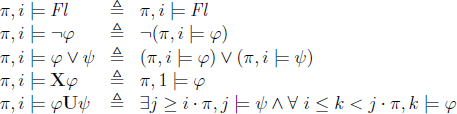
\includegraphics{Imagenes/Otros/ltl.png}
	\caption{Semántica para el operador de satisfacción $\vDash$}
	\label{fig:ltl}
\end{figure}

Dada una traza infinita $\pi$, la satisfacción de una formula $\varphi$ en la posición $i$, denotada $\pi, i\vDash \varphi$ se define como en la figura 2.1.
Decimos que $\varphi$ se sostiene en $\pi$ si $\pi, 0\vDash \varphi$. Una formula $\varphi \in FLTL$ se sostiene en un LTS $E$ si se sostiene en cada traza
infinita producida por $E$.

\end{definition}


\section{Generalised Reactivity (1)}

Dada una secuencia infinita de estados, una formula GR(1) denota cuales han ocurrido infinitamente. 
Más formalmente, $\phi = (A, B)$ en donde $A$ y $B$ son conjuntos de subconjuntos de estados en donde o bien alguno de los
subconjuntos de $A$ no contiene ningún estado que se visita infinitamente, o bien todos los subconjuntos de $B$ contienen 
al menos un estado que se visita infinitamente.

\begin{definition}{(Generalised Reactivity (1))}
Sea $Estados$ el conjunto universal de estados. Dada una secuancia infinita de estados $p$, sean $inf(p)$ los estados que
ocurren infinitamente en $p$. Sea $\phi_{1}, ..., \phi_{n}$ y $\varUpsilon_{1}, ..., \varUpsilon_{m}$ subconjuntos de $Estados$. Sea\\
$gr((\phi_{1}, ..., \phi_{n}), (\varUpsilon_{1}, ..., \varUpsilon_{m}))$ el conjunto de infinitas secuencias $p$ tales que
o bien para algun $i$ vale $inf(p)\cap\phi_{i} = \varnothing$ o para todo $j$ vale $inf(p)\cap\varUpsilon_{j} \neq \varnothing$
\end{definition}

\section{Síntesis de controladores}

La síntesis de controladores se encarga de producir automáticamente una máquina que restringe la ocurrencia de eventos
controlables basándose en la observación de los eventos que ya ocurrieron. Cuando esta máquina es desplegada en un ambiente
adecuado garantiza la satisfacción de un conjunto de objetivos dado. La satisfacción de estos objetivos depende de la
satisfacción de las asunciones sobre el entorno.

\subsection{LTS control problem}

Podemos describir la síntesis de controladores de la siguiente forma. Dados un LTS que describe el comportamiento
del entorno, un conjunto de acciones controlables, un conjunto de fórmulas FLTL que representan las suposiciones
del dominio y un conjunto de fórmulas FLTL que representan los objetivos del sistema, el problema de control de
LTS \cite{LTSControl} es encontrar un LTS que solo restrinja la ocurrencia de acciones controlables y garantice que la composición
en paralelo entre el ambiente y el LTS es deadlock free y que si las suposiciones de dominio se satisfacen, entonces
los objetivos del sistema también son satisfechos.

\begin{definition}{(LTS control)}
Dado un modelo del domino en forma de un LTS determinístico $E = (S_{E}, A_{E}, \Delta_{E}, s_{0}^{E})$, un conjunto de
acciones controlables $A_{c} \subseteq A_{E}$ y una formula FLTL $\varphi$, la solución al LTS control problem
$\varepsilon = \langle E, \varphi, A_{c} \rangle$ es un LTS $M = (S_{M}, A_{M}, \Delta_{M}, s_{0}^{M})$ tal que
$A_{M} = A_{E}$, y por cada estado en $S_{M}$ todas las acciones en $A_{M} \setminus A_{c}$ estás habilitadas, $E \parallel M$
es deadlock free, y toda traza $\pi$ en $E \parallel M$ garantiza $\pi \vDash \varphi$
\end{definition}

El LTS Control Problem es decidible en tiempo exponencial y en caso de ser decidible, se encuentra la solución con la
misma complejidad. Para esto es necesario que el modelo sea determinístico.

\subsection{MTS	control problem}

El problema de la síntesis de controladores para MTSs \cite{MTSControl} consiste en ver si todas, alguna o ninguna de sus implementaciones
pueden ser controladas por un controlador LTS. Al responder esta pregunta, también estamos respondiendo la pregunta de
si el problema es realizable, ya que si la respuesta es ninguno el problema no es realizable. Para decidir este problema,
primero se intenta encontrar un controlador para la implementación del MTS que tiene todas las acciones posibles controlables.
Si se lo encuentra, se tiene un controlador para todas las posibles implementaciones. Se hace lo mismo con el que tiene la
mínima cantidad de acciones controlables y así se obtiene la respuesta.

\begin{definition}{(MTS control)}
Dado un modelo del domino en forma de un MTS $M = (S_{M}, A, \Delta_{M}^{r}, \Delta_{M}^{p}, s_{0}^{M})$, un conjunto de
acciones controlables $A_{c} \subseteq A_{M}$ y una formula FLTL $\varphi$, la solución al MTS control problem
$\varepsilon = \langle M, \varphi, A_{c} \rangle$ es responder:

\begin{itemize}

\item
\textbf{All} si para todo LTS $I$ que sea implementación de $M$, el LTS control problem $\langle I, \varphi, A_{c} \rangle$ es realizable.

\item
\textbf{None} si para ningún LTS $I$ que sea implementación de $M$, el LTS control problem $\langle I, \varphi, A_{c} \rangle$ es realizable.

\item
\textbf{Some} en otro caso.

\end{itemize}

\end{definition}